
\chapter{Grundlagen}
\label{ch:Grundlagen}


\section{ABB - DE-IS}

ABB ist ein global f\"{u}hrender Hersteller und Serviceanbieter in der Energie- und Automatisierungstechnik mit Hauptsitz in Z\"{u}rich.
Der internationale Konzern entstand 1988 aus der Fusion des schwedischen Unternehmens \ac{ASEA} und der schweizerischen Firma \ac{BBC}. ABB besch\"{a}ftigt zurzeit \"{u}ber 132.000 Mitarbeiter in 100 L\"{a}ndern. Im Jahr 2016 wurde ein weltweiter Umsatz von 33,8 Mrd. USD und ein Nettogewinn von 2,1 Mrd erwirtschaftet.\footnote{Vgl. ABB Gesch\"{a}ftsbericht 2016} 
\linebreak



\begin{figure}[ht]
	\centering
	\makebox[\textwidth][c]{
\includegraphics[width=1\textwidth]{img/ABB-Div.png}}%
	
	\caption{Divisionen von ABB}
	\label{fig1}
	
\end{figure}

Das Produktportfolio von ABB gliedert sich in vier Divisionen auf: Division Electrification, Robotics and Motion, Industrial Automation und Power Grids. Diese Aufteilung ist auch in Abbildung \ref{fig1} zu sehen.

Der Bereich \ac{DE-IS} fungiert als Koordinator der IT-Kernfunktionen der ABB Deutschland, sowie teilweise für Zentraleuropa. In enger Zusammenarbeit mit den operativen Einheiten werden unter anderem folgende Aufgaben wahrgenommen:

\begin{itemize}
	\item Vertretung der ABB in Deutschland gegenüber diversen Serviceprovidern wie beispielsweise der IBM
	\item Unterstützung des operativen Geschäfts mit Hilfe von informationstechnischen sowie applikativen  Lösungen sowie der Betreuung dieser.
	\item Verwaltung laufender IS-Betriebsprozesse in Abstimmung mit den IS-Verantwortlichen vor Ort
	\item Administration und Erweiterung des \ac{ERP}-Systems der ABB AG
\end{itemize}


\section{SAP}
SAP SE ist ein deutsches Software-Unternehmen mit Sitz in Walldorf. Als viertgrößter Softwareanbieter der Welt beschäftigt das Unternehmen weltweit mehr als 84 Tausend Mitarbeiter. SAP hat sich auf Ressourcenmanagement-Software spezialisiert. Das Hauseigene \ac{ERP}-System "`SAP"' findet in fast 50\% aller Unternehmen mit mehr als 500 Mitarbeitern Anwendung. Ein \ac{ERP}-System ist dafür da, Betriebswirtschaftliche Prozesse zu bündeln und verwalten. Dabei werden alle unternehmensrelevanten Ressourcen wie Personal, Kapital und Material geplant sowie gesteuert. 

ABB nutzt als \ac{ERP} System die Standardsoftware SAP R/3. Eine Standardsoftware ist ein Produkt, welches die allgemeinen Anforderungen des Nutzers - in diesem Fall ABB - erfüllt und bei speziellen Anforderungen individuell angepasst werden kann. Die Firma SAP SE bietet verschiedene Modulare Lösungen an, welche einzeln genutzt werden können. Beispiele sind hierfür die \ac{SD}-, \ac{FI}-, \ac{MM}- und \ac{HR}-Module. 

SAP SE hat eigens für ihr \ac{ERP}-System die Programmiersprache \ac{ABAP} entwickelt. Grundsätzlich ist \ac{ABAP} eine Mischung aus \ac{SQL}- und Java-Befehlen. Dabei ist  die Programmiersprache so optimiert, effizient mit großen Datenbanken gearbeitet werden kann. In den letzten Jahren wurde \ac{ABAP} in sofern weiterentwickelt, dass nun auch objektorientiertes Arbeiten ermöglicht wird. SAP ist zum größten Teil mit \ac{ABAP} programmiert, sodass Anpassungen und eigene Programme auch in \ac{ABAP} geschrieben werden müssen. 




\section{Interactive Forms by Adobe}

Seit 2002 arbeitet SAP mit der Software Firma Adobe zusammen, um eine neue Art der Dokumenten-Erstellung im SAP zu schaffen. Aus dieser Zusammenarbeit entstanden die "`Interactive Forms by Adobe"', welche seit Jahren den Standard für die PDF\footnote{\ac{PDF} ist ein plattformunabhängiges Dateiformat, entwickelt von Adobe}-Erstellung in SAP bilden. Trotz dessen, wird diese Technologie bei ABB erst seit kurzem eingesetzt.

Neue PDF-Dokumente können größtenteils ohne Programmieraufwand erstellt bzw. angepasst werden. Als Hauptwerkzeug dient hierbei der Adobe Lifecycle Designer, welcher mit Hilfe von grafischen Darstellungen einfacheres Arbeiten ermöglicht.

   

Die Erstellung von Adobe PDFs in SAP besteht aus drei Teilen:

\begin{itemize}
	\item Eine Schnittstelle, in welcher die Daten und Einstellungen der PDF festgelegt sind.
	\item Das eigentliche Formular, welches das Layout sowie den Inhalt des Dokumentes vorgibt.
	\item Ein Druckprogramm, welches die Schnittstelle mit dem Formular verbindet und die PDF druckt.
\end{itemize}

\subsection{Technischer Aufbau der Adobe \ac{PDF}}

Adobe Forms sind ähnlich unterteilt wie der Vorgänger Smart Forms. Es gibt eine Schnittstelle, in welcher die Datendefinition und die Formularlogik festgelegt werden. Zum einen sind hier die Import- und Export-Parameter für den Dokumentendruck definiert und zum anderen die tatsächlichen Daten, mit welchen das Formular gefüllt wird. Zusätzlich wird noch die Möglichkeit gegeben, die Daten mit Hilfe von \ac{ABAP}-Code bei der Initialisierung der Dokumentenerstellung anzupassen.

Neben der Schnittstelle gibt es noch das eigentliche Formular. Jedes Formular muss einer Schnittstelle zugewiesen sein. Nur dann sind die in der Schnittstelle definierten Felder benutzbar. Hier ist zu beachten, dass mehrere Formulare die selbe Schnittstelle nutzen können. \footnote{Vgl. \cite{Hauser.2015} S.125-128} 

Im Formular wird zuerst ausgewählt, welchen Anteil der Daten, der in der Schnittstelle hinterlegt ist, im Dokument verwendet wird und unter welchen Bedingungen diese ausgegeben werden. Erste Eigenschaften der Felder im Dokument müssen schon hier bestimmt werden wie beispielsweise, ob das Feld aktiv ist oder nicht.

Beim Aktivieren des Formulars wird im Hintergrund ein Funktionsbaustein erstellt, welcher die Schnittstelle zwischen der Datenbeschaffung und Ausgabe des Formulars darstellt. Ein Funktionsbaustein ist ein in sich selbst abgeschlossenes Teilprogramm, welches mit oder ohne Input-Parameter ausgeführt werden kann. Dieser ist vor allem für Funktionen hilfreich, welche oft in verschiedenen Situationen in SAP genutzt werden.

\subsection{Aufbau eines Adobe Formulars}

Die Erstellung eines Dokumentes im Form Builder ist in zwei Teile gespalten, dem "Kontext" sowie dem Layout. 

Im Kontext Bereich stehen die Inhalte der konfigurierten Schnittstelle zur Auswahl. Aus dieser Auswahl wird eine Datenhierarchie festgelegt. Nur diese Inhalte stehen im nächsten Teil, dem Layout, zu Verfügung. Sollen bestimmte Teile des Dokumentes nur unter bestimmten Bedingungen angezeigt werden, können diese Einstellungen ebenfalls im Kontext Bereich vorgenommen werden. Bei bestimmten Inhalten der PDF können bzw. müssen gewisse Eigenschaften festgelegt werden.
 Elemente der PDF welche beispielsweise abhängig von der Sprache sind, müssen einen Wert für die zu verwendete Sprache beinhalten. In Abbildung \ref{figAD} ist dies für das Beispiel der Adressfelder zu sehen. Bei Adressfeldern ist die Ausgabe relevant vom Absender-Land.
 
 \begin{figure}[ht]
 	\centering
 	\makebox[\textwidth][c]{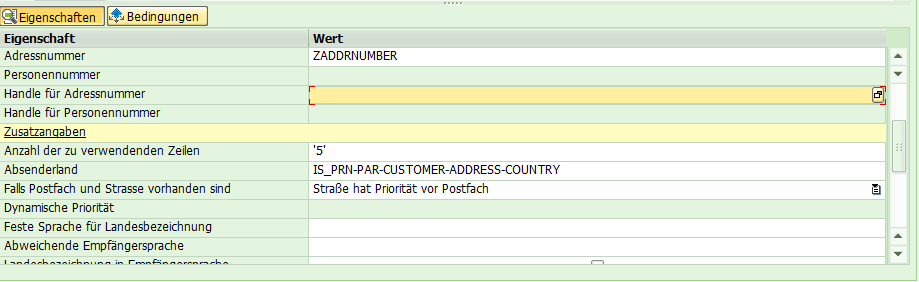
\includegraphics[width=1\textwidth]{img/Adressfeld.png}}%
 	
 	\caption{Eigenschaften eines Adressfeldes}
 	\label{figAD}
 	
 \end{figure}

Unabhängig von den Daten aus der Schnittstelle können zusätzliche Objekte wie Abbildungen und Textbausteine hinzugefügt werden. Der tatsächliche Inhalt dieser Objekte kann wiederum abhängig von den Schnittstellendaten sein. Somit bildet der Kontext das Bindeglied zwischen den Formulardaten und dem Dokumenten Layout.\footnote{Vgl. \cite{Hauser.2015} S.145-146} 

Eingebettet in das SAP \ac{GUI} ist der \ac{ALCD}. Mit Hilfe dieses Tools wird die Formularvorlage für den Druck einer Adobe PDF erstellt. Auf Basis der, im Kontext definierten, Daten wird somit das Layout des Formulars sowie der anzuzeigende Inhalt festgelegt. Folgende Funktionen sind hierbei Schlüsselwerkzeuge bei der Erstellung eines Dokumentes. \footcite{Hauser.2015}

\begin{itemize}
	\item Hierarchie und Datenansicht \\
		Diese zwei Baumartigen Darstellungen stellen unterschiedliche Aspekte des Formulars dar. Die Hierarchie zeigt den strukturellen Aufbau des Dokuments während die Datenansicht den Aufbau der Daten visualisiert.
	\item Bibliothek \\
		Die Bibliothek bildet eine Ansammlung von Feldtypen welche Standardmäßig für ein Dokument zur Verfügung stellen. Oft verwendete Felder, wie beispielsweise Bild- oder Text-Felder können somit leichter genutzt werden.
	\item Objekt-Palette \\
		In den verschiedenen Reitern der Objekt-Palette werden die Eigenschaften von Formularfeldern festgelegt.
	\item Formulardesignfläche \\
		Diese Fläche bildet den Hauptbereich des \ac{ALCD} da hier die Konfiguration der Formularvorlage stattfindet. Unterteilt wir sie in die Designansicht, welche das Layout der einzelnen Seiten definiert, und den Masterseiten, welche die Hintergrunde sowie das Format der Designseiten vorgibt.
	\item Datenbindungen \\
		Mit Hilfe der Objekt-Palette werden Feldern eine Datenbindung zugewiesen. Über diese Bindung wird definiert, welche Daten in dem jeweiligen Feld angezeigt werden.
	\item Felder im Fließtext \\
		Dynamische Inhalte, welche im Fließtext vorkommen, werden mit dieser Funktion eingefügt. Diese Felder werden beim Drucken der PDF gefüllt und der Fließtext um das Feld herum wird dementsprechend angepasst.
	\item Tabellen \\
		Da die Größe von Tabellen meistens erst zum Zeitpunkt des Druckes feststeht muss eine dynamische Ausgabe möglich sein. Mit dieser Funktion können Tabellen erstellt und die Ausgaberegeln festgelegt werden.
	\item Seitenumbrüche \\
		Bei Dokumenten mit dynamischen Inhalten ist es mit Hilfe dieser Funktion möglich, bedingte Seitenumbrüche festzulegen um gegebenenfalls Inhalte auf einer beliebigen Anzahl neuer Seiten mit einem festgelegten Layout darzustellen.
\end{itemize} 
       

\FloatBarrier
\section{Langzeit-Lieferantenerklärung}

 Lieferantenerklärungen (LE) sind Dokumente, welche bei einer Lieferung Auskunft bezüglich des Herkunftslandes beinhaltender Waren gibt. Diese Angaben werden bei verschiedenen Zollprozessen benötigt. Grundsätzlich wird die \ac{LE} bei Warenbewegungen innerhalb der \ac{EU} verwendet. Die \ac{LLE}, welche als Beispiel-Dokument für diese Arbeit benutzt wird, ist eine einmalige Erklärung welche für gleiche Lieferungen über einen maximalen Zeitraum von 2 Jahren gilt.\footcite{ZOLL.2017} 2016 erstellte ABB alleine in Deutschland dieses Dokument 1800 mal.\footnote{Nach Internen Auswertungen} Text und Aufbau der \ac{LLE} entsprechen gesetzlichen Vorgaben. Dementsprechend wird in der folgenden Arbeit nur auf die technische Umsetzung der selbigen eingegangen.
